\Chapter{Related Work}\label{chapter:related}

In this chapter, I provide a comprehensive review of existing approaches relevant to novel view synthesis from single or few input images. The chapter begins by introducing the fundamental task of Novel View Synthesis (NVS) and its significance in computer vision and 3D understanding. We then examine traditional 3D reconstruction techniques (Section \ref{sec:3d-reconstruction}) and their inherent limitations, particularly for sparse-input scenarios, which motivates the exploration of generative methods. Subsequently, the discussion shifts to the foundational principles of Deep Generative Models for Image Synthesis, with a focus on diffusion models (Section \ref{sec:text-to-image}).

Building on this foundation, we explore various methods for Conditioning Diffusion Models for Enhanced Control and Adaptation to New Tasks (Section \ref{sec:conditioning-diffusion}), including crucial techniques for camera parameter encoding and lightweight adaptation mechanisms. The core of the chapter then examines state-of-the-art Diffusion-based Novel View Synthesis techniques (Section \ref{sec:novel-view-diffusion}), covering both single-image novel view synthesis and architectures for coherent multi-view generation.

\section{Traditional 3D Reconstruction Approaches}\label{sec:3d-reconstruction}

Before examining generative approaches to novel view synthesis, it is essential to understand the limitations of traditional 3D reconstruction methods that motivate the shift toward diffusion-based solutions.

\begin{figure}[h]
  \centering
  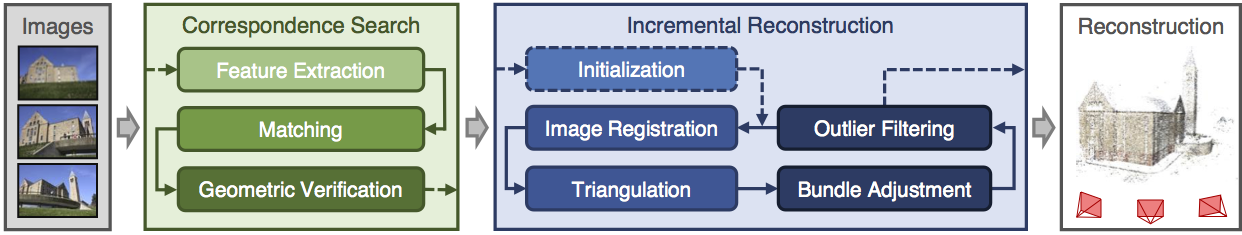
\includegraphics[width=0.9\textwidth]{images/related-work/COLMAP.png}
  \caption{COLMAP pipeline (Source:\cite{colmap_figure})}
  \label{fig:colmap-pipeline}
\end{figure}
Structure from Motion (SfM) represents the classical approach to 3D reconstruction from images. Methods like COLMAP \cite{colmap} demonstrate remarkable success in reconstructing 3D scenes from dense image collections through a two-stage pipeline \ref{fig:colmap-pipeline}: correspondence search to identify and match features across images, followed by incremental reconstruction to estimate camera poses and triangulate 3D points.

\begin{figure}[h]
  \centering
  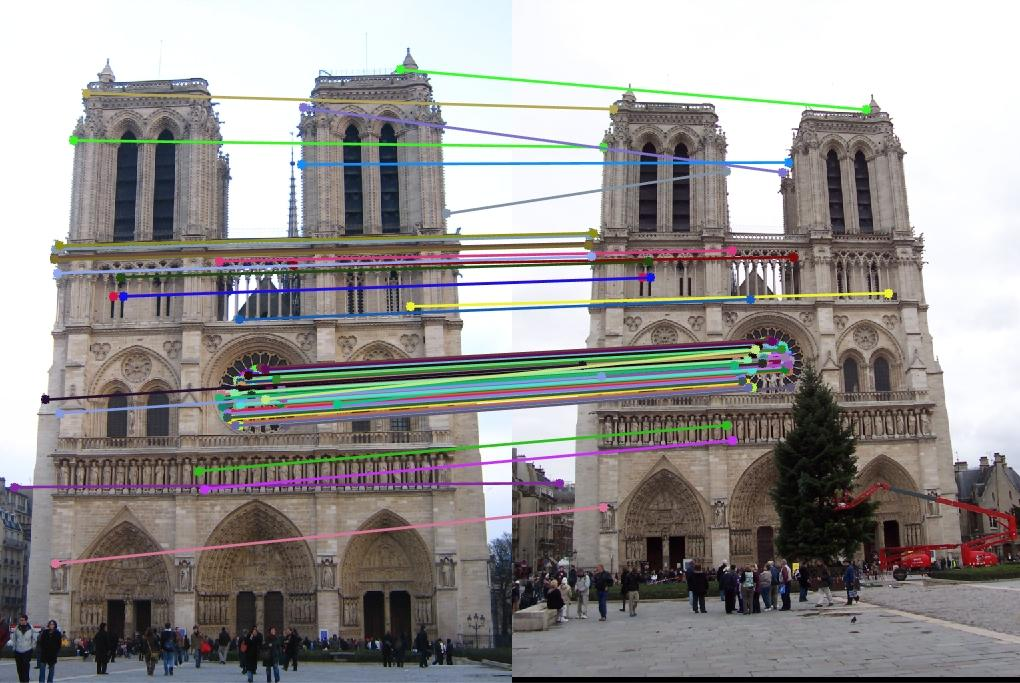
\includegraphics[width=0.7\textwidth]{images/related-work/feature-matching.jpg}
  \caption{Feature matching across multiple views - a fundamental requirement for traditional SfM approaches (Source:\cite{image_matching})}
  \label{fig:matching-features}
  % https://blog.roboflow.com/image-matching/
\end{figure}

The success of SfM relies heavily on several key components: robust feature detection (typically using SIFT \cite{sift} or ORB \cite{orb}), accurate feature matching across viewpoints, and bundle adjustment to refine camera poses and 3D points. Dense reconstruction methods like Multi-View Stereo (MVS) can then generate detailed 3D models from the sparse SfM output.

More recent learning-based approaches, including Neural Radiance Fields (NeRF) \cite{nerf}, have shown remarkable results for novel view synthesis. NeRF represents scenes as continuous 5D functions encoded in neural networks, taking camera poses from SfM as input and using volume rendering to synthesize photorealistic novel views with impressive detail and view consistency.

\subsection{Fundamental Limitations for Sparse Input Scenarios}

Traditional 3D reconstruction methods face critical limitations when applied to sparse input scenarios - particularly the extreme case of single-image novel view synthesis that forms the focus of this thesis:

\begin{enumerate}
  \item \textbf{Insufficient correspondences}: SfM requires reliable feature matches across multiple views. With only one or very few images, establishing robust correspondences becomes impossible.

  \item \textbf{Geometric ambiguity}: Single images provide incomplete depth information and cannot resolve occlusions, leading to fundamental ambiguities in 3D structure.

  \item \textbf{View-dependent effects}: Materials with specular reflections or varying appearance cannot be accurately modeled without observing them from multiple known viewpoints.

  \item \textbf{Scale and pose estimation}: Without multiple views, determining absolute scale and object pose becomes severely under-constrained.
\end{enumerate}

These limitations have motivated the development of generative approaches to novel view synthesis, particularly using diffusion models trained on large datasets of 3D assets. Instead of explicitly reconstructing geometry through correspondences, these methods leverage the power of deep learning to learn and synthesize plausible views from learned priors about object appearance and structure.

Modern 3D generation pipelines, such as InstantMesh \cite{instantmesh}, exemplify this paradigm shift by using diffusion models for multi-view generation as a first step, followed by 3D reconstruction from the synthesized views.

\begin{figure}[h]
  \centering
  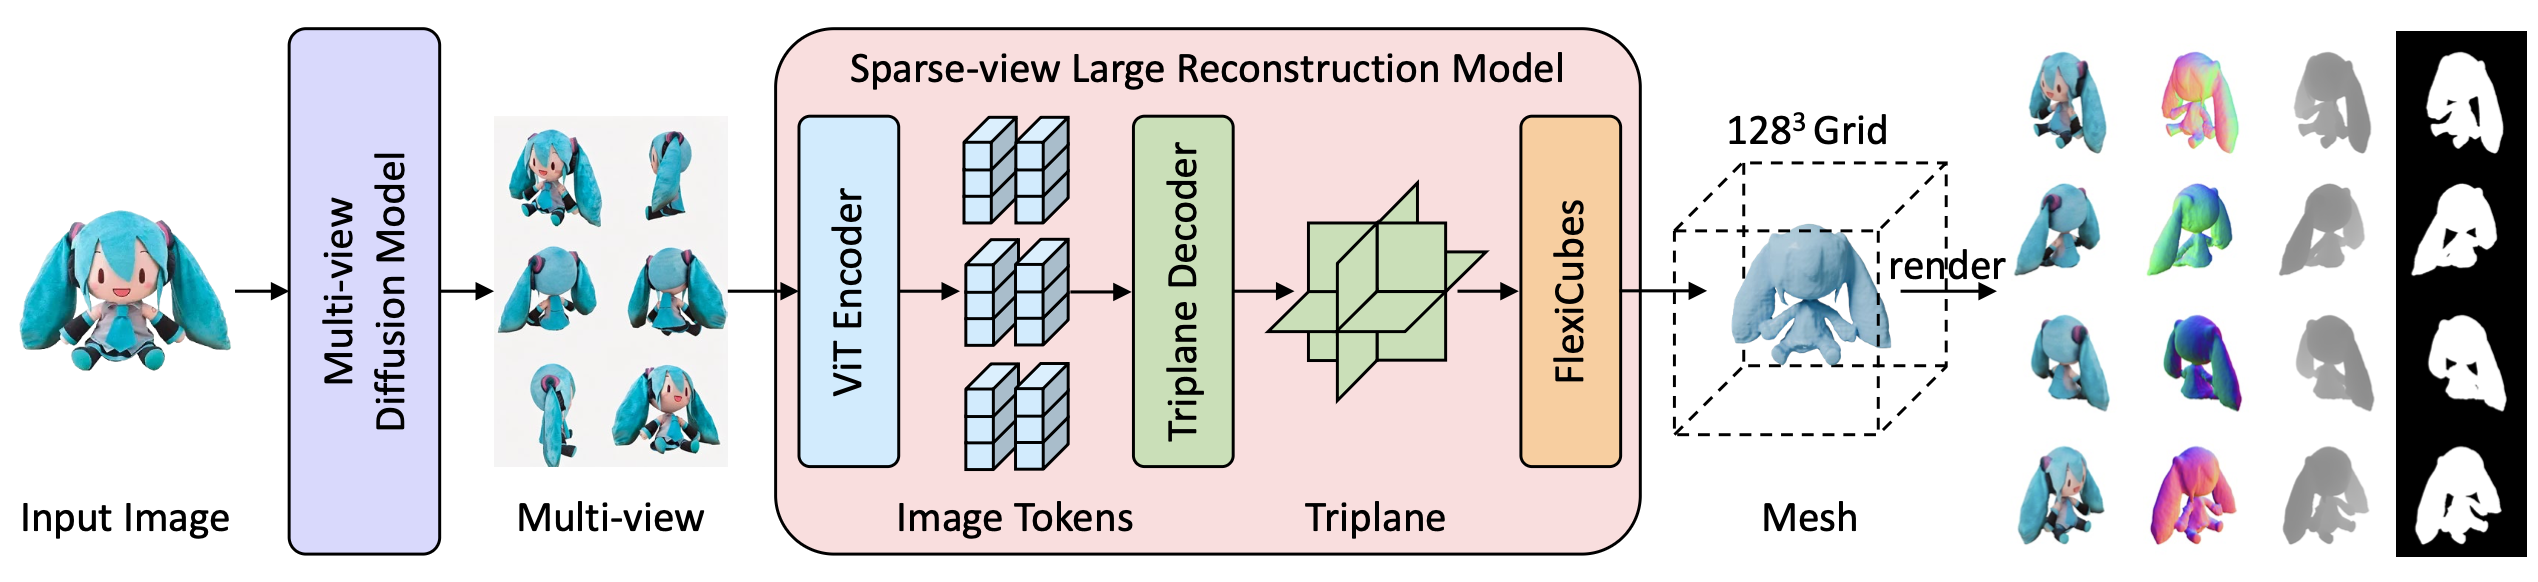
\includegraphics[width=\textwidth]{images/related-work/instantmesh.png}
  \caption{InstantMesh pipeline showing novel view synthesis as the foundation for 3D reconstruction (Source:\cite{instantmesh})}
  \label{fig:instantmesh}
\end{figure}

This transition from geometric reconstruction to generative synthesis motivates the focus of this thesis on developing efficient and effective diffusion-based approaches for novel view synthesis.

\section{Deep Generative Models for Image Synthesis}\label{sec:text-to-image}

The development of deep learning methods has led to remarkable progress in generative modeling, enabling the synthesis of highly realistic and diverse images. Among the various approaches, Generative Adversarial Networks (GANs), Variational Autoencoders (VAEs), and Diffusion Models have emerged as the most prominent. While GANs and VAEs have laid significant groundwork and continue to be influential, this section will primarily focus on diffusion models, given their state-of-the-art performance in image quality and controllability, and their direct relevance to the multi-view synthesis tasks explored in this thesis.

\subsection{Generative Adversarial Networks and Variational Autoencoders}

Generative Adversarial Networks (GANs) \cite{gan} consist of two neural networks, a generator and a discriminator, trained in a competitive setting. The generator aims to produce realistic images, while the discriminator tries to distinguish between real images from the training dataset and fake images produced by the generator. Through this adversarial process, the generator learns to create increasingly plausible images. GANs are known for generating sharp images but often suffer from training instability.

Variational Autoencoders (VAEs) \cite{vae} are another class of generative models that learn a probabilistic mapping from a high-dimensional data space (e.g., images) to a lower-dimensional latent space, and then back to the data space. A VAE consists of an encoder that compresses the input data into a latent representation (typically a mean and variance defining a Gaussian distribution) and a decoder that reconstructs the data from samples drawn from this latent distribution. They are trained to maximize the evidence lower bound (ELBO), which involves a reconstruction loss and a regularization term (KL divergence) that encourages the latent space to be smooth and well-behaved. VAEs generally offer more stable training than GANs and can learn a meaningful latent space, but often produce slightly blurrier images. VAEs play a crucial role in the architecture of Latent Diffusion Models.

\subsection{Diffusion Models}
Diffusion models have recently become the dominant paradigm in high-fidelity image generation. They are inspired by non-equilibrium thermodynamics, specifically diffusion processes.

\subsubsection{The Diffusion Process}
The core idea behind diffusion models involves two processes: a forward (or diffusion) process and a reverse (or denoising) process.
In the \textbf{forward process}, a known image $x_0$ from the dataset is gradually perturbed by adding small amounts of Gaussian noise over a sequence of $T$ steps. This process progressively corrupts the image until, at step $T$, it becomes indistinguishable from pure isotropic Gaussian noise. The parameters of this noising process are fixed.

The \textbf{reverse process} aims to learn to reverse this noising. Starting from pure noise (equivalent to $x_T$), a neural network is trained to gradually denoise the signal, step-by-step, eventually producing a realistic image (an approximation of $x_0$). This learned denoising process is what allows the model to generate new images. Figure \ref{fig:diffusion-process} illustrates this concept.

\begin{figure}[h]
  \centering
  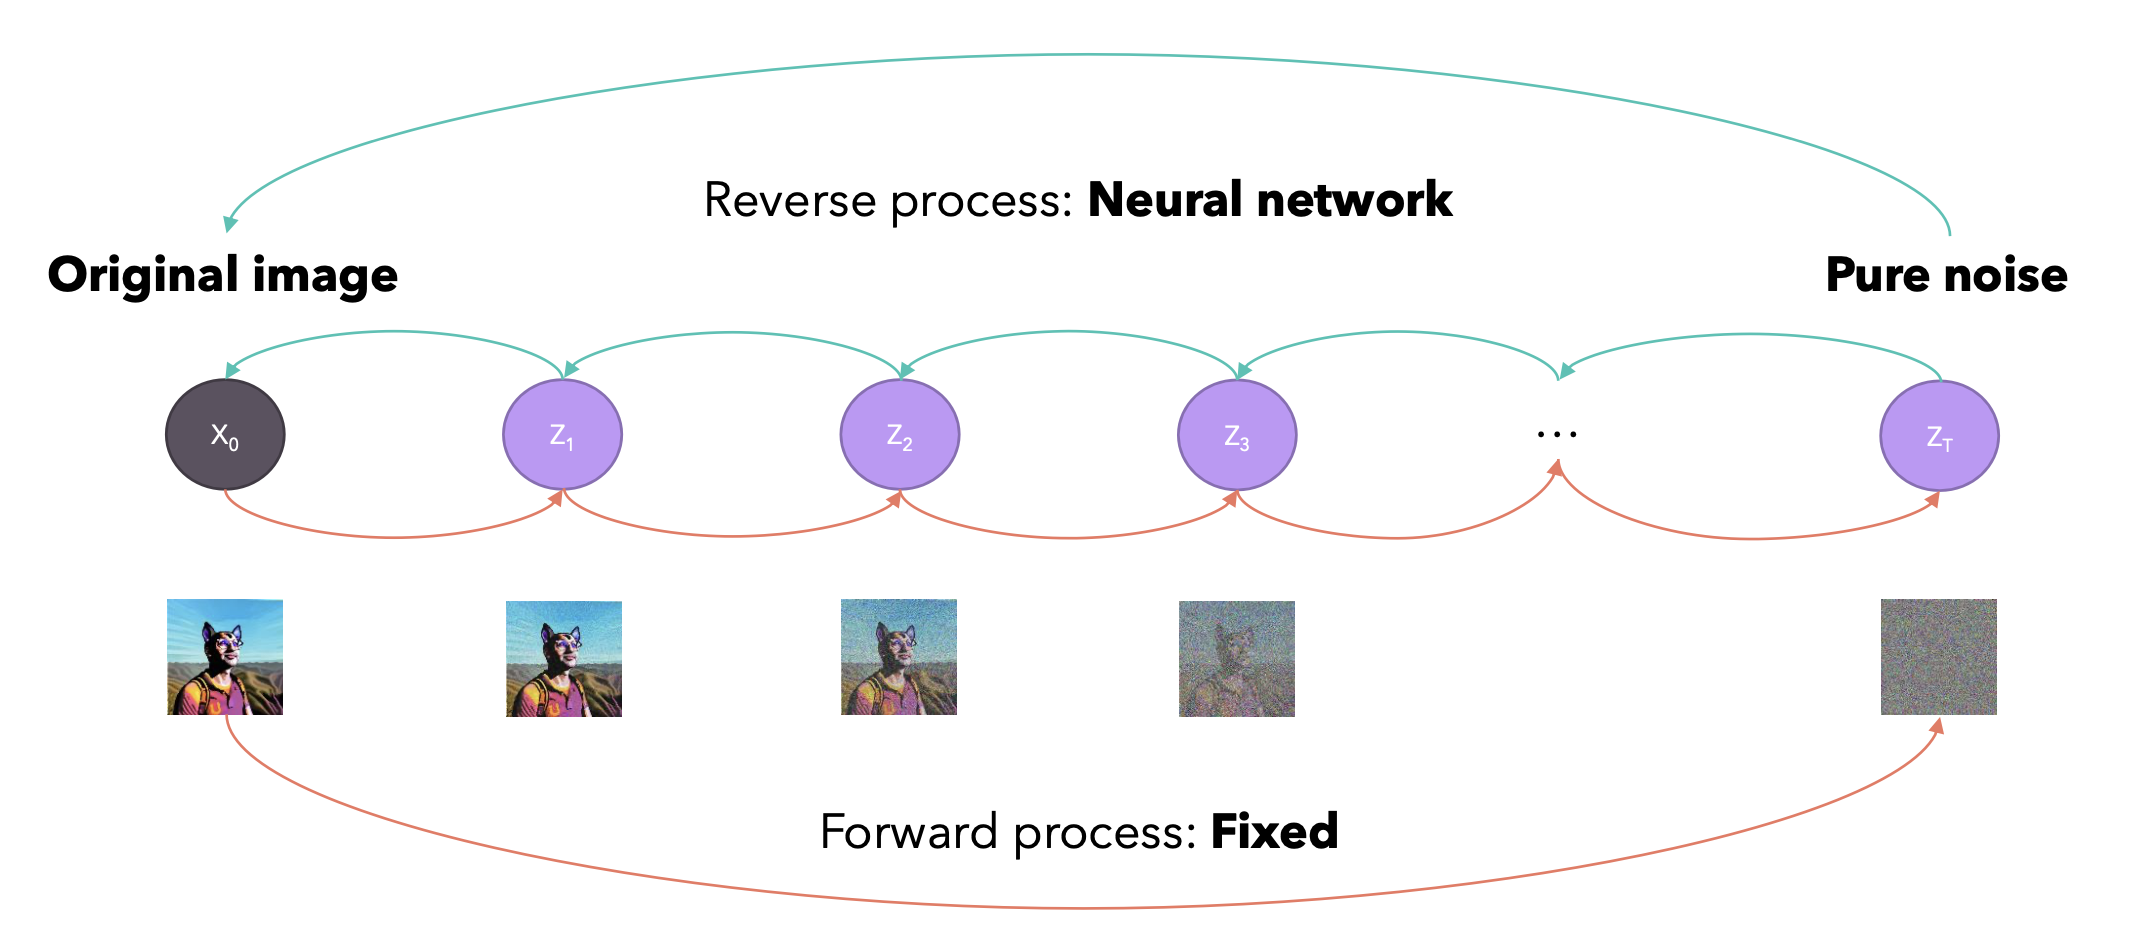
\includegraphics[width=0.8\textwidth]{images/related-work/diffusion-process.png}
  \caption{The forward (noising) and reverse (denoising/generation) stages of a diffusion model. The forward process gradually adds noise to an image until it becomes pure noise. The reverse process learned by a neural net to denoise, step-by-step, to generate an image from noise. (Source:\cite{diffusion_process})}
  \label{fig:diffusion-process}
\end{figure}

\subsubsection{The U-Net Architecture}
The neural network responsible for predicting the noise (or the denoised image) at each step in the reverse process is typically a U-Net architecture \cite{unet}. The U-Net, originally developed for biomedical image segmentation, features an encoder-decoder structure with skip (residual) connections. The encoder path progressively downsamples the input, capturing contextual information, while the decoder path progressively upsamples, localizing information. The skip connections concatenate features from the encoder to corresponding layers in the decoder, allowing the network to combine high-level semantic information with low-level detail, which is crucial for accurately predicting the noise and preserving image fidelity during the denoising steps.

\subsubsection{Training Objective and Loss Function}
The training objective of the diffusion model is to learn the conditional probability distribution $p_\theta(x_{t-1}|x_t)$, which represents the probability of the previous, less noisy state $x_{t-1}$ given the current noisy state $x_t$. In practice, this is often simplified to training the U-Net to predict the noise $\epsilon$ that was added to an image $x_0$ to produce $x_t$ at a given timestep $t$. The loss function is typically the Mean Squared Error (MSE) between the true added noise $\epsilon$ and the noise $\epsilon_\theta(x_t, t)$ predicted by the U-Net:
\[ L = \mathbb{E}_{t \sim [1, T], x_0 \sim q(x_0), \epsilon \sim \mathcal{N}(0, I)} [\|\epsilon - \epsilon_\theta(x_t, t)\|^2] \]
where $x_t = \sqrt{\bar{\alpha}_t}x_0 + \sqrt{1-\bar{\alpha}_t}\epsilon$, and $\bar{\alpha}_t$ are parameters from the noise schedule.

\subsubsection{Conditional Generation: Text-to-Image Synthesis}
To guide the image generation process, diffusion models can be conditioned on various inputs, most notably text prompts. This is the foundation of text-to-image synthesis.
A crucial component for text conditioning is a powerful text encoder that can convert textual descriptions into rich numerical representations (embeddings). Contrastive Language-Image Pre-training (CLIP) \cite{clip} is widely used for this purpose. CLIP is trained on a massive dataset of image-text pairs to learn a shared embedding space where semantically similar images and texts are close together.

The text embeddings from CLIP are then integrated into the U-Net, typically using cross-attention mechanisms. In these layers, the image representation at an intermediate layer of the U-Net queries the text embedding, allowing the model to align parts of the image with relevant words or phrases in the prompt. This enables fine-grained control over the generated image content based on the textual input.

\subsection{Latent Diffusion Models (LDMs)}\label{ssec:ldm}
While standard diffusion models operate directly in the pixel space of images, this can be computationally very expensive, especially for high-resolution images, as the U-Net needs to process large tensors. Latent Diffusion Models (LDMs) \cite{stablediffusion}, such as Stable Diffusion, address this challenge by performing the diffusion and denoising process in a lower-dimensional latent space.

LDMs employ a pre-trained autoencoder, typically a VAE. The VAE's encoder first compresses a high-resolution image from pixel space into a compact latent representation. The diffusion process (both forward and reverse) then occurs entirely within this latent space. Once the reverse denoising process generates a target latent representation from noise, the VAE's decoder maps this latent representation back into the high-resolution pixel space to produce the final image. Figure \ref{fig:ldm-architecture} depicts the architecture of an LDM.

\begin{figure}[h]
  \centering
  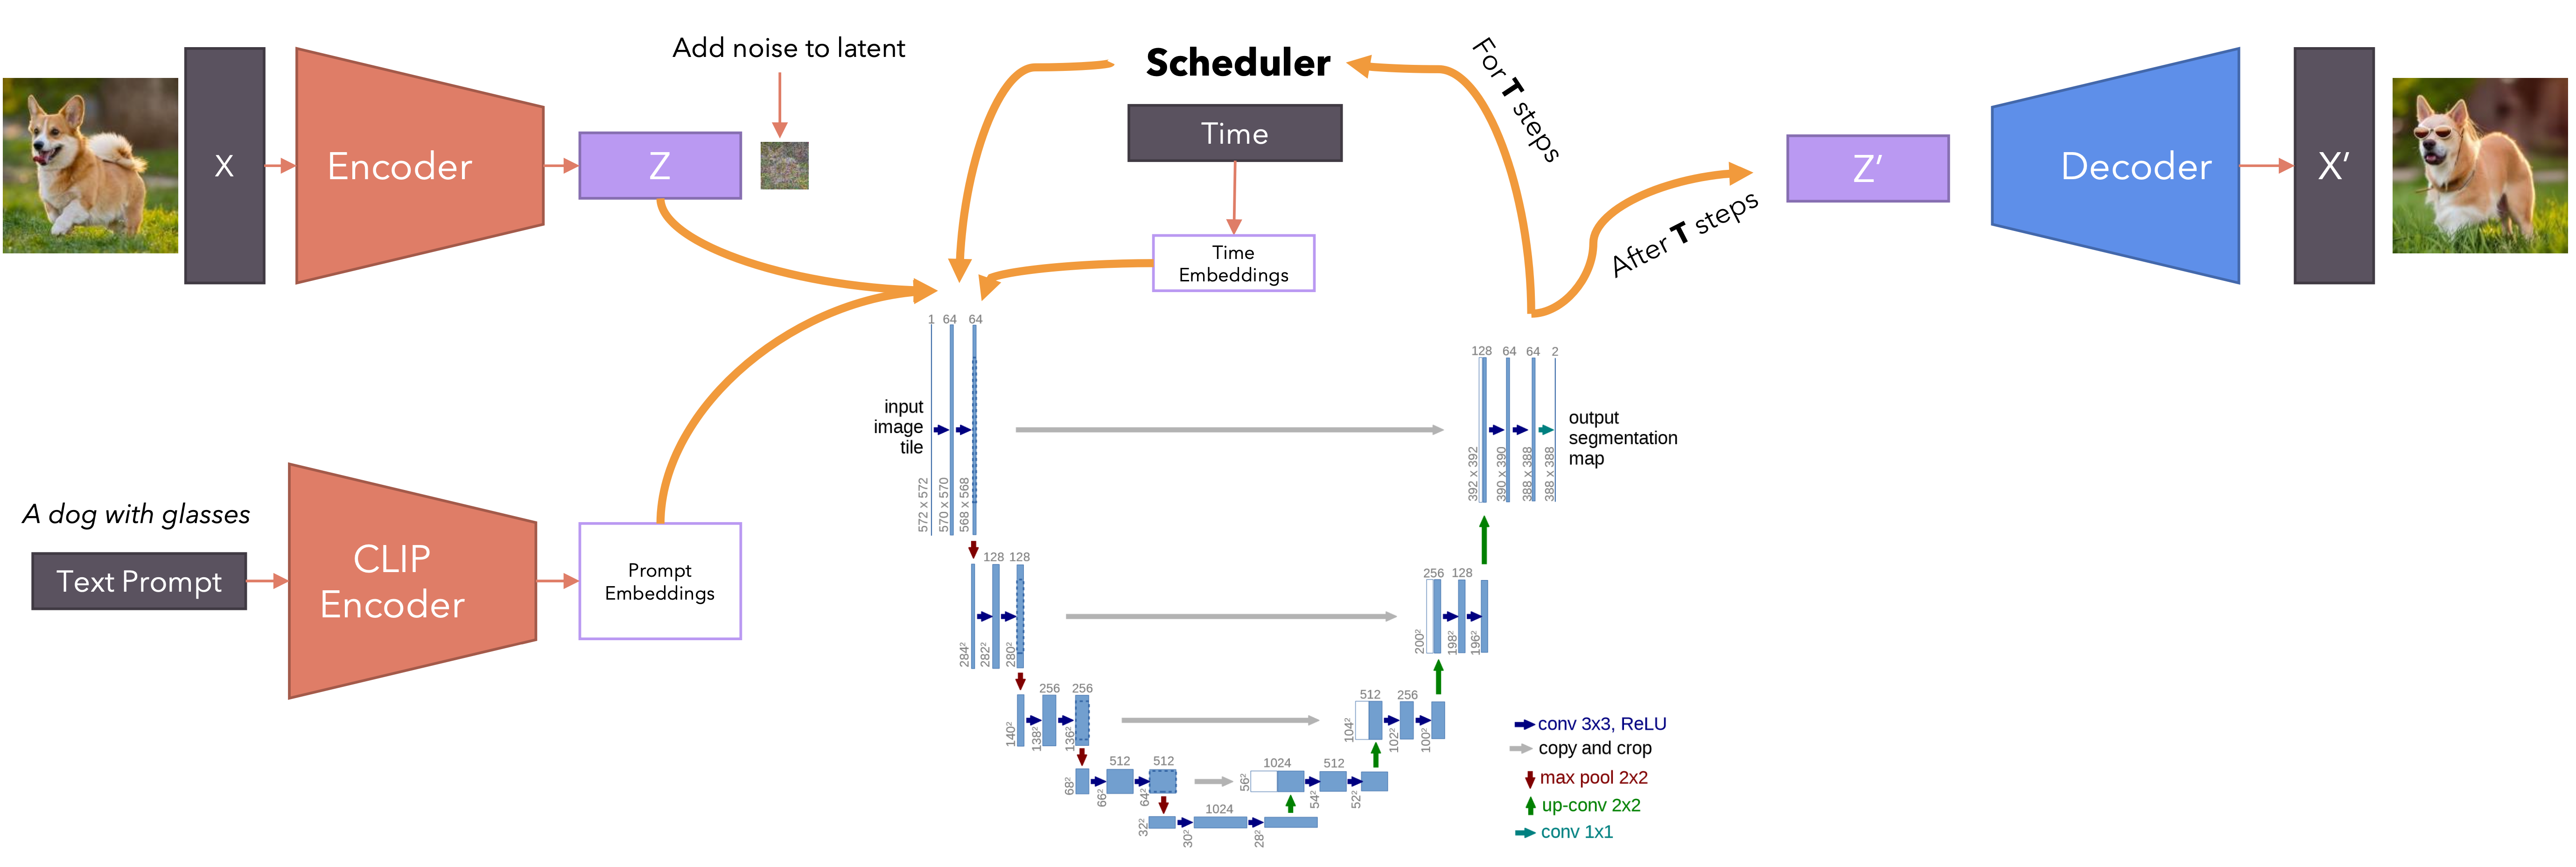
\includegraphics[width=\textwidth]{images/related-work/LDM-detailed.png}
  \caption{Architecture of a Latent Diffusion Model (LDM). An image is first encoded into a latent space by a VAE encoder. The diffusion process (noising and denoising via U-Net) occurs in this latent space. The generated latent is then decoded back to pixel space by the VAE decoder. Conditioning, such as text embeddings from CLIP, is incorporated into the U-Net. (Source:\cite{diffusion_process})}
  \label{fig:ldm-architecture}
\end{figure}

By working in a compressed latent space, LDMs significantly reduce the computational burden during training and inference compared to pixel-space diffusion models. This makes it feasible to train powerful models on massive datasets and generate high-resolution images more efficiently, without a substantial loss in quality. The VAE ensures that the latent space is perceptually equivalent to the pixel space, and the diffusion model learns to generate high-quality latents within this space.

\section{Conditioning Diffusion Models for Enhanced Control and New Tasks}\label{sec:conditioning-diffusion}

While textual prompts provide a powerful and intuitive way to guide diffusion models, the generation process can be conditioned on a much wider array of signals. This opens up possibilities for more fine-grained control over the output and enables new applications beyond text-to-image synthesis. This section explores several advanced conditioning mechanisms, focusing on image-based conditioning for detailed content and style control, and specialized techniques for incorporating geometric information, such as camera parameters, to enrich 2D diffusion models with 3D awareness.

\subsection{Image-based Conditioning for Fine-Grained Control}
Conditioning on reference images allows for precise control over spatial layout, object appearance, color consistency, or artistic style, going beyond what is often achievable with text alone.

\subsubsection{ControlNet}
ControlNet \cite{controlnet} introduces a method to add diverse spatial conditioning to pre-trained text-to-image diffusion models. Instead of fine-tuning the original large model, ControlNet involves training smaller, task-specific auxiliary networks that are attached to the frozen U-Net backbone of the diffusion model, typically to its encoder blocks. These auxiliary networks take an input conditioning image (e.g., an edge map, human pose skeleton, depth map, or segmentation map) and produce feature maps that are then added to the corresponding features of the main U-Net. This approach allows the pre-trained model to be guided by the spatial information in the conditioning image while retaining its vast generative capabilities learned from large datasets. The original U-Net weights are locked, making ControlNet modules efficient to train and portable. Figure \ref{fig:controlnet-overview} provides a conceptual overview.

\begin{figure}[ht]
  \centering
  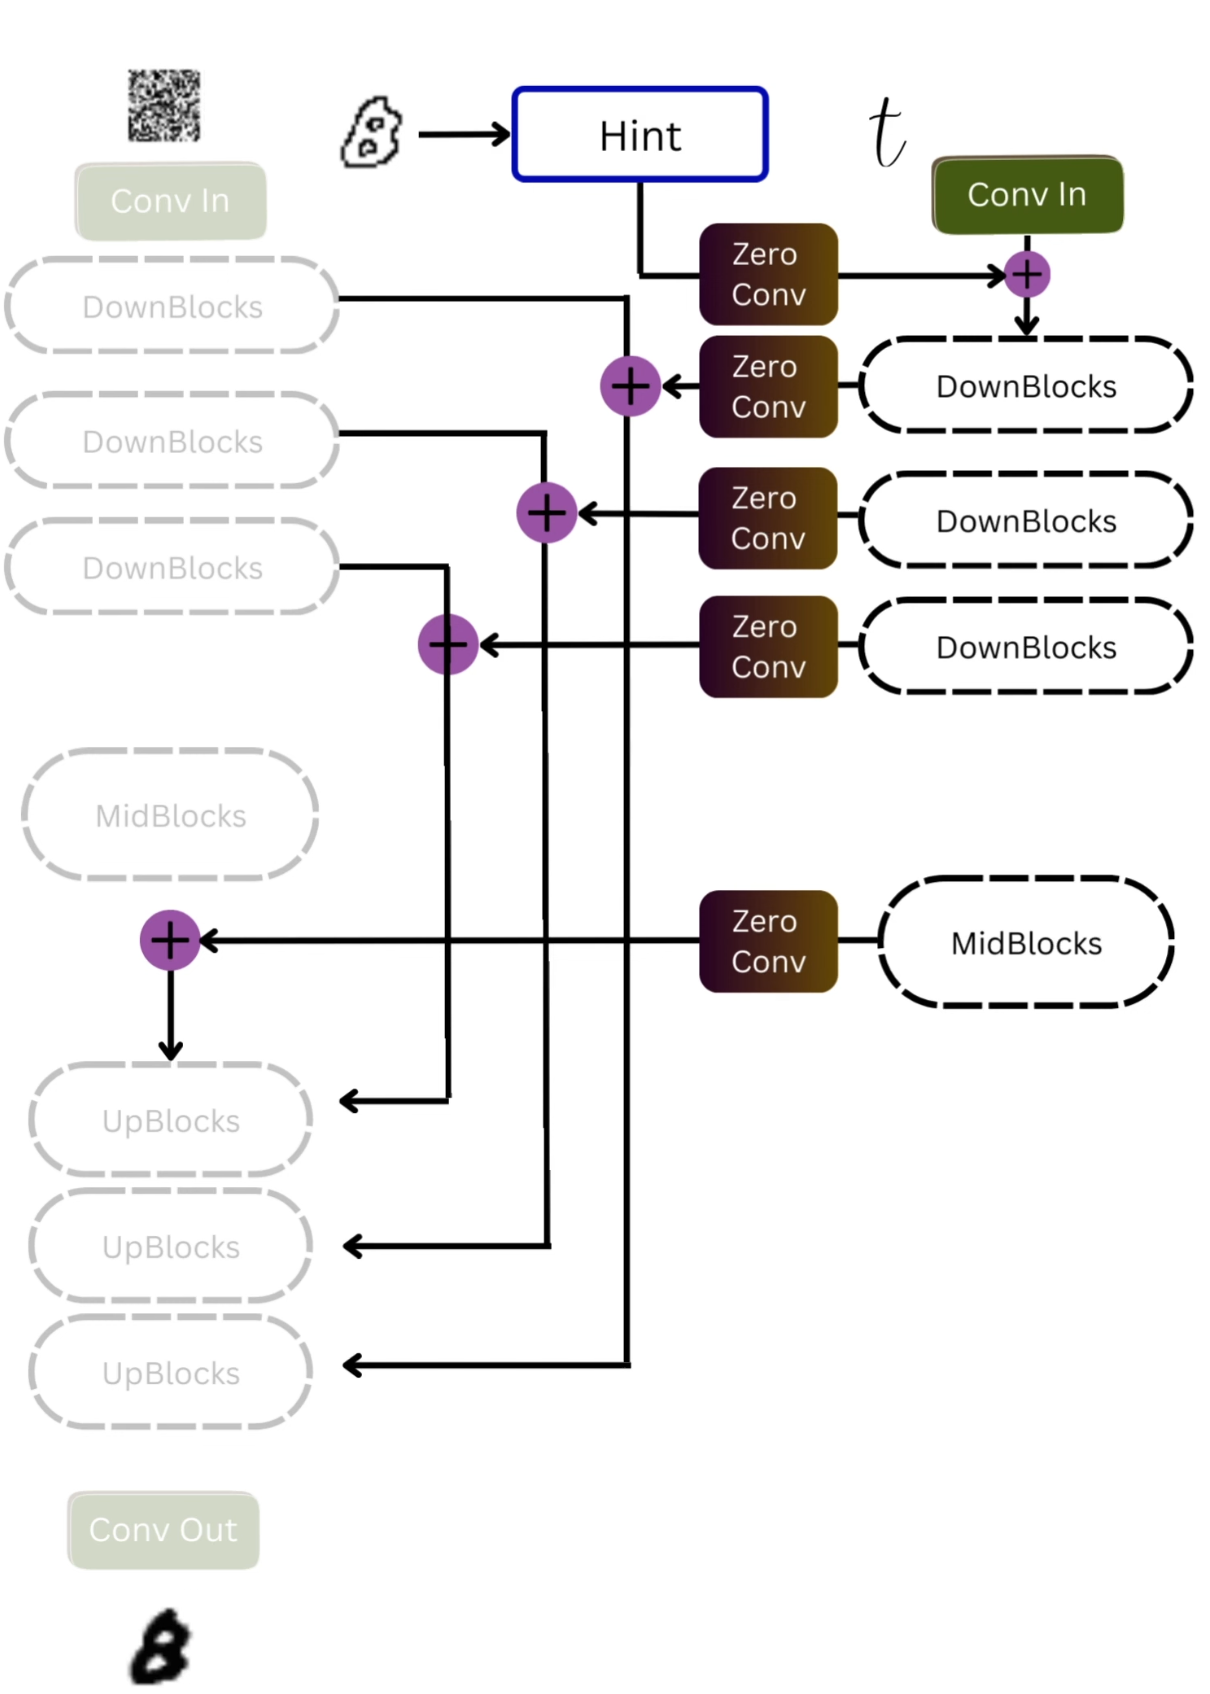
\includegraphics[width=0.4\textwidth]{images/related-work/controlnet.png}
  \caption{Conceptual overview of ControlNet, showing how an additional control module processes an input condition (e.g., edges, pose) and injects guidance into a pre-trained diffusion model. (Adapted from Zhang et al. \cite{controlnet}) (Source:\cite{controlnet_figure})}
  \label{fig:controlnet-overview}
\end{figure}

\subsubsection{IP-Adapter}
IP-Adapter (Image Prompt Adapter) \cite{ipadapter} offers an effective way to condition diffusion models using an image prompt, allowing the model to generate images that align with the content or style of the reference image. It achieves this by introducing a lightweight adapter module that can be plugged into a pre-trained text-to-image model. The core idea is to decouple the cross-attention mechanisms used for text and image features. Image features, extracted by an image encoder (like CLIP \cite{clip} image encoder), are fed into new cross-attention layers that work in parallel with the original text cross-attention layers. This allows the model to draw information from both text and image prompts simultaneously or prioritize one over the other. IP-Adapter is efficient as it avoids fine-tuning the large base model and only trains the adapter parameters, making it a versatile tool for tasks like style transfer or subject-driven generation. Figure \ref{fig:ipadapter-concept} illustrates this concept.

\begin{figure}[h]
  \centering
  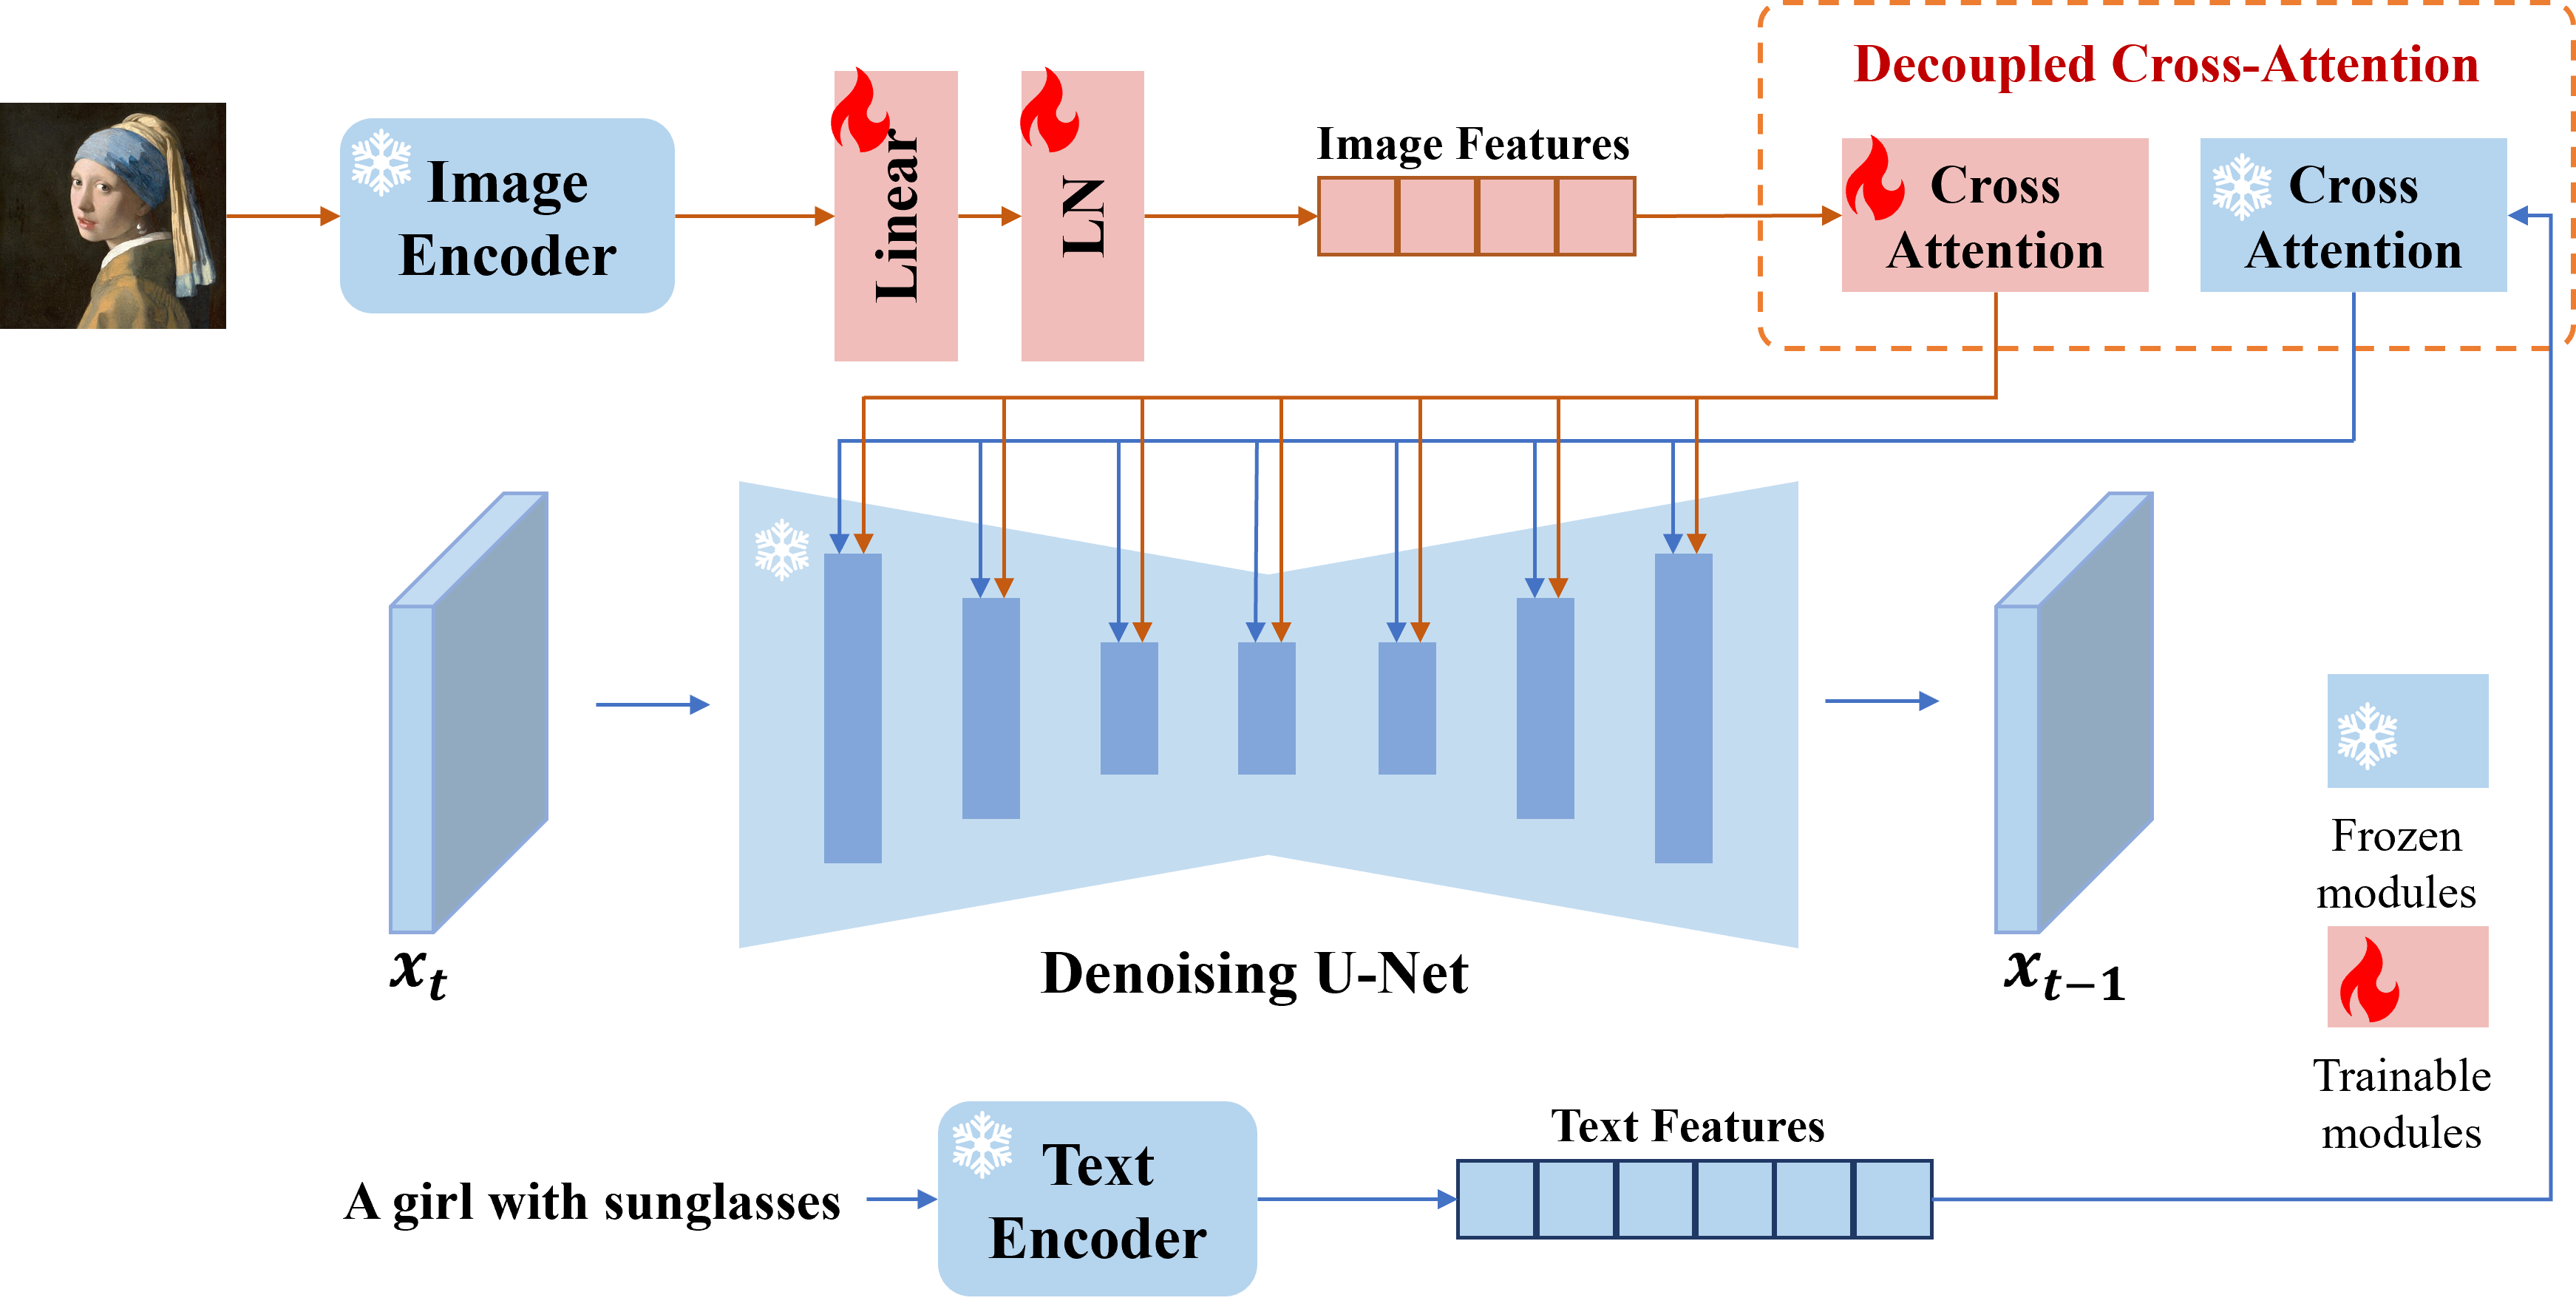
\includegraphics[width=0.7\textwidth]{images/related-work/ipadapter.png}
  \caption{Conceptual illustration of the IP-Adapter architecture, showing how image features extracted by an image encoder are integrated into the U-Net via dedicated cross-attention layers to guide the generation process. (Image based on the IP-Adapter concept) (Source:\cite{ipadapter})}
  \label{fig:ipadapter-concept}
\end{figure}

\subsubsection{CatVTON and UNet Feature Conditioning}
A particularly relevant approach for image conditioning, especially for tasks requiring detailed transfer of appearance or garment characteristics, is found in methods like CatVTON \cite{catvton}. The key insight in such methods is to leverage the rich, hierarchical features learned by the denoising U-Net itself. When provided with a reference image (e.g., an image of a specific garment), features can be extracted from various layers of the U-Net as it processes this reference. These extracted features, which encode information about texture, shape, and style at multiple scales, are then used to condition the generation of a new image (e.g., the same garment, but worn by a person). This conditioning can be achieved by injecting these features into the corresponding layers of the U-Net during the denoising process of the target image, often using attention mechanisms or direct feature fusion. This technique allows for a powerful form of image-based control that is highly attuned to the diffusion model's internal representations, facilitating tasks like virtual try-on with impressive fidelity by directly utilizing the U-Net's understanding of visual elements.

\subsection{Modulating Network Activations}
Feature-wise Linear Modulation (FiLM) \cite{film} is a general and effective technique for conditioning neural network activations. Instead of directly concatenating conditioning information or using complex gating mechanisms, FiLM applies a simple affine transformation to feature maps based on a conditioning input. Given a feature map $h$ from a layer in a neural network, and a conditioning vector $c$, a FiLM generator (typically a small neural network) produces a scale parameter $\gamma$ and a shift parameter $\beta$ from $c$. These parameters then modulate $h$ as follows: $FiLM(h) = \gamma \cdot h + \beta$. This allows the conditioning information $c$ to dynamically influence the behavior of the network layer by layer. FiLM is lightweight and can be integrated into various architectures to allow secondary inputs to control the processing of a primary input. Figure \ref{fig:film-layer} illustrates the internals of a FiLM layer.

\begin{figure}[h]
  \centering
  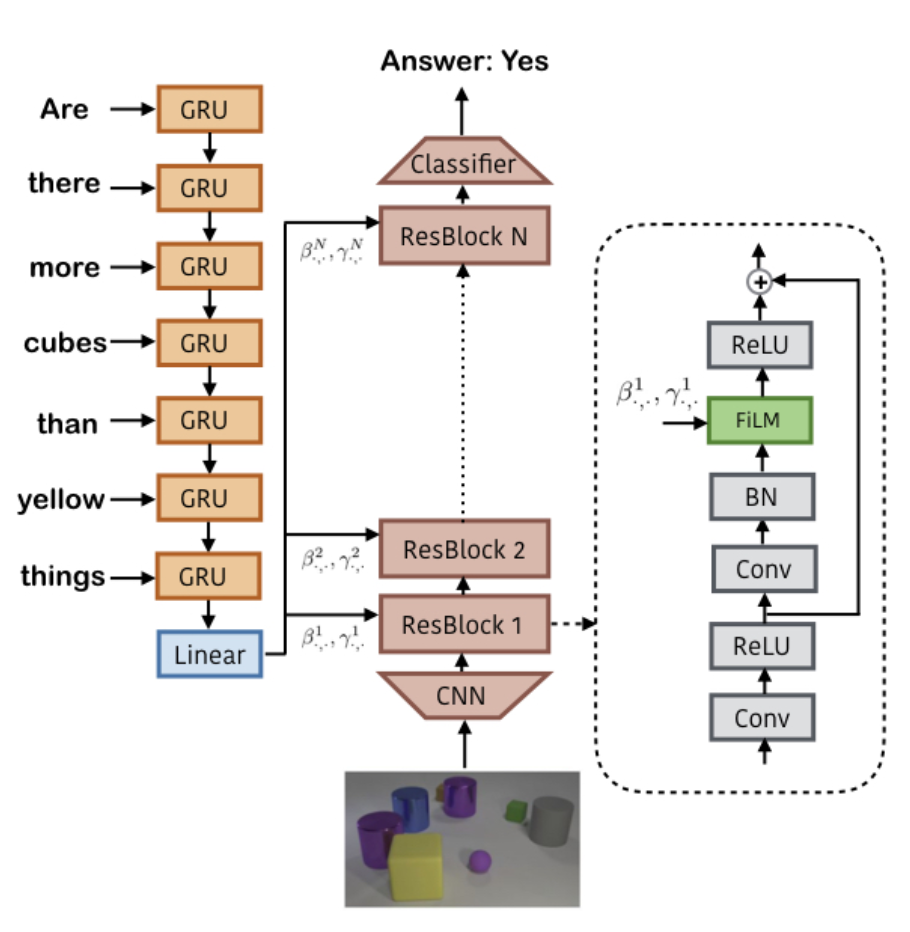
\includegraphics[width=0.5\textwidth]{images/related-work/film.png}
  \caption{The Feature-wise Linear Modulation (FiLM) layer. A conditioning input is processed by a FiLM generator to produce scale ($\gamma$) and shift ($\beta$) parameters, which then modulate the feature maps ($h$) of a main network. (Adapted from Perez et al. \cite{film}) (Source:\cite{film})}
  \label{fig:film-layer}
\end{figure}

This approach enabled image-based models to effectively integrate and act upon conditioning information from outside the image domain. For instance, by modulating visual features based on encoded text tokens, it empowered (at the time) state-of-the-art image question answering models to ground their visual processing in textual context.

\subsubsection{FiLMed-UNet}
The FiLM technique has also been effectively applied to U-Net architectures in the medical imaging domain, notably in the FiLMed-UNet paper by Lemay et al. \cite{filmedunet}. Their work focused on enhancing medical image segmentation by incorporating various forms of metadata as conditioning signals. FiLMed-UNet utilized patient-specific information, such as tumor type or the target organ for segmentation.

The core idea was to make the U-Net's segmentation process adaptable and more informed by this external metadata. The metadata (e.g., one-hot encoded tumor type) was passed through a FiLM generator network, which produced scale ($\gamma$) and shift ($\beta$) parameters. These parameters then modulated the feature maps at different layers within the U-Net. This allowed the network to tailor its feature extraction and segmentation logic based on the provided metadata. For example, knowing the tumor type allowed the model to leverage type-specific visual characteristics, leading to improved segmentation accuracy. Furthermore, by conditioning on the desired output class (e.g., "segment kidney"), FiLMed-UNet demonstrated robustness in multi-task learning scenarios, even with missing labels for some tasks in the training data, and showed improved performance with limited annotations. While this application of FiLM is distinct from encoding camera parameters for 3D-aware synthesis, it highlights the versatility of FiLM in allowing neural networks to integrate and utilize diverse conditioning information to adapt their behavior for specialized tasks. Figure \ref{fig:filmed-unet-concept} shows a conceptual diagram.

\begin{figure}[h]
  \centering
  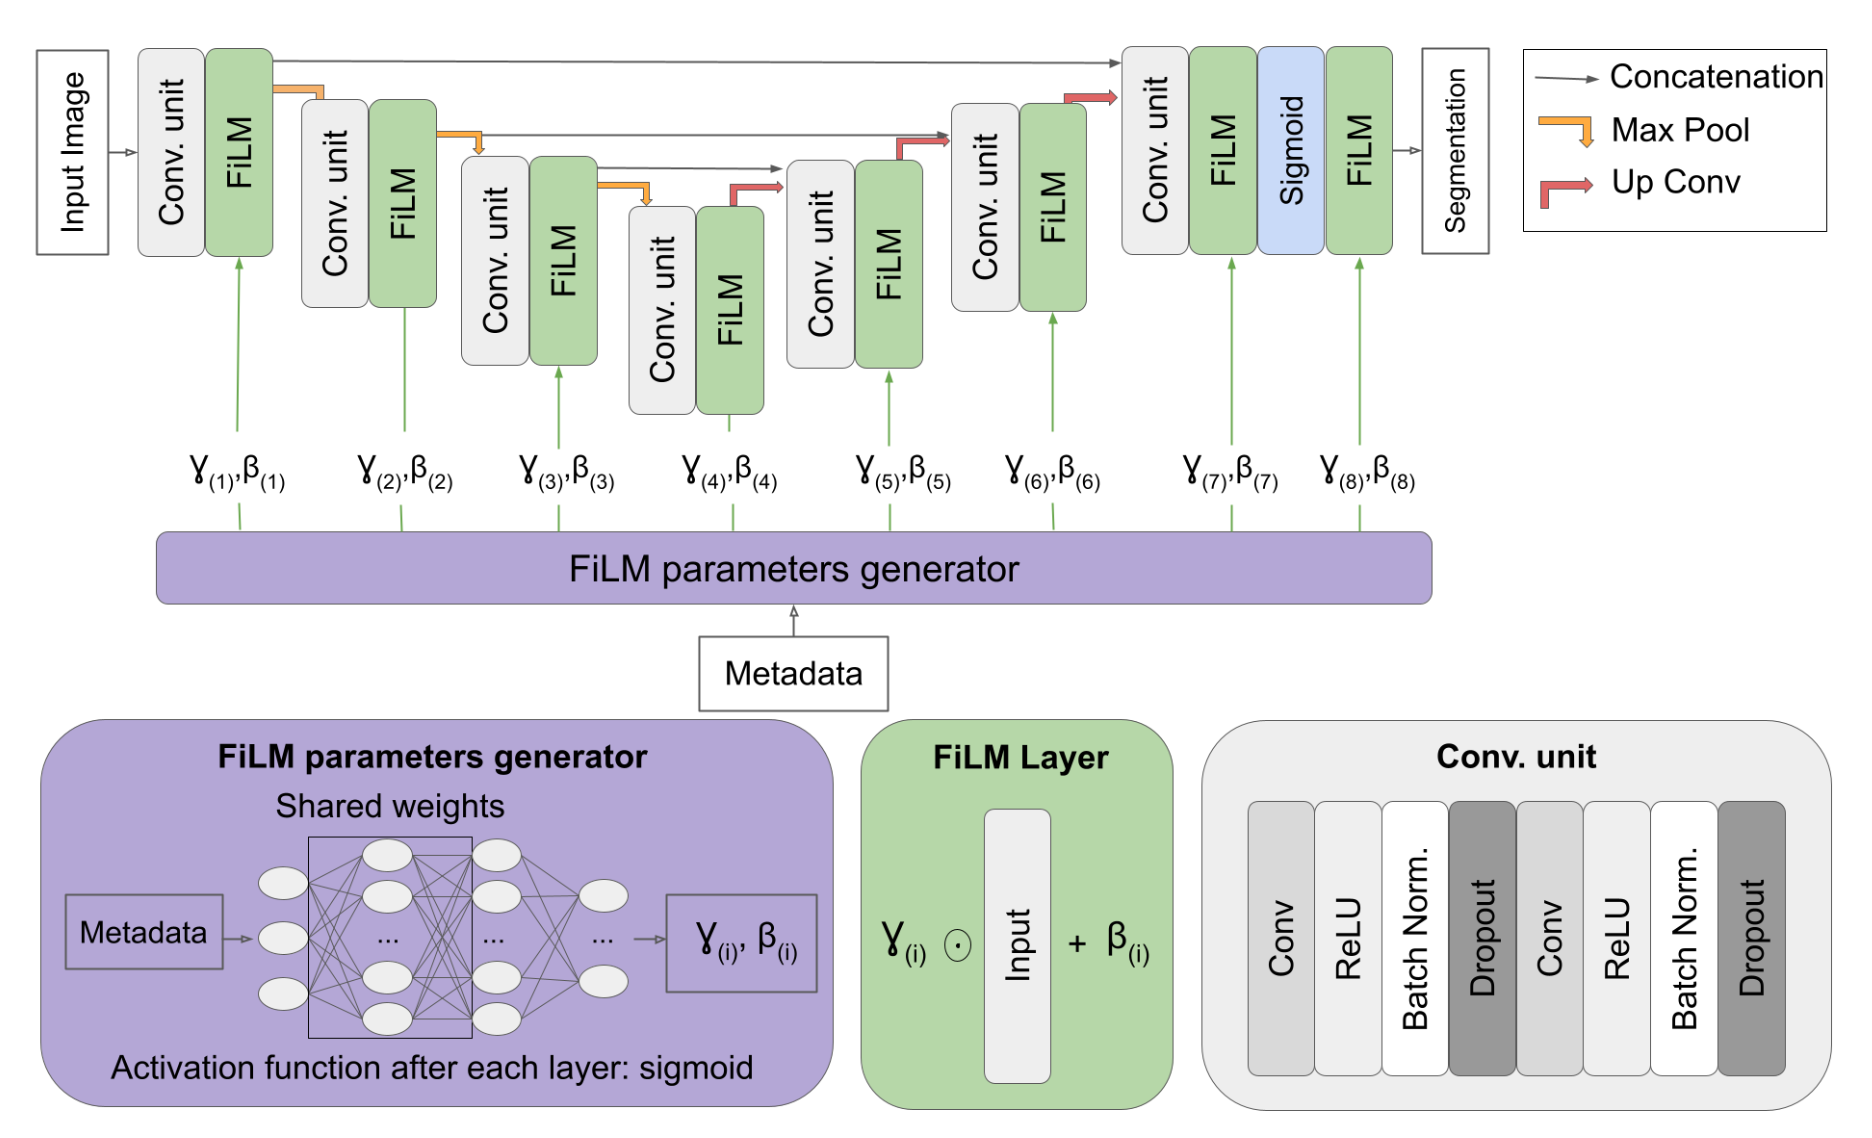
\includegraphics[width=0.7\textwidth]{images/related-work/filmed-unet.png}
  \caption{Conceptual diagram of a FiLMed-UNet. The metadata about patients are processed by a FiLM generator network, which outputs scale and shift parameters to modulate activations at various layers within the U-Net architecture, making the denoising process viewpoint-aware. (Source:\cite{filmed_unet})}
  \label{fig:filmed-unet-concept}

\end{figure}

\subsection{Camera Parameter Encoding for 3D Awareness}\label{ssec:camera_param_encoding}
Making 2D diffusion models inherently 3D-aware is crucial for tasks like multi-view image generation. A key aspect of this is encoding camera parameters (Rotation R, Translation t) to guide the image generation process. Various methods focus on integrating this geometric information directly into the model's input or intermediate representations.

\subsubsection{Pixel-Level Geometric Conditioning: Ray-based Approaches}
This category of methods aims to provide detailed, per-pixel geometric information derived from camera parameters directly to the diffusion model.
A prominent technique is the use of a \textit{raymap}, as demonstrated by Watson et al. \cite{novelviewsynthesisdiffusion} in 3DiM and also utilized in CAT3D \cite{cat3d}. The raymap is a tensor with the same spatial dimensions as the image or latent representation. At each (u,v) coordinate, it stores the 3D origin and 3D direction of the camera ray passing through that pixel. In CAT3D, these rays are computed relative to the camera pose of the first conditional image.
To help the network learn high-frequency details associated with viewpoint changes, these ray origins and directions are often further processed using positional encodings.
The resulting positionally encoded raymap can be concatenated as an additional input channel to the U-Net, alongside the noisy image or latent representation \cite{novelviewsynthesisdiffusion, cat3d}. This allows the model to learn a direct, spatially varying mapping from ray geometry to the target pixel output.
% CAT3D \cite{cat3d} notes that such raymap conditioning generalizes better than using low-dimensional vector embeddings for camera pose, particularly for out-of-domain samples.

\subsubsection{Global Camera Pose Conditioning}
Alongside per-pixel data, global camera pose conditioning methods provide a more compact, holistic representation of the camera's viewpoint or transformation.
One approach involves \textit{vectorized transformation embeddings}. For instance, Zero-1-to-3 \cite{zero1to3} encodes the relative camera viewpoint transformation \(T = [R|t]\) between an input view and a target view as a 4x4 matrix. This matrix is flattened into a 16-dimensional vector, which is then projected by a small Multi-Layer Perceptron (MLP) and added to the timestep embedding. This globally influences the diffusion process by providing context about the desired viewpoint change.
Another technique employs \textit{decomposed pose vectors for attention mechanisms}. MV-Adapter \cite{mvadapter} represents each camera view using a 12-dimensional vector, which includes 3D camera coordinates and a 9D flattened rotation matrix. These vectors are processed by an MLP and then fed into multi-view attention layers as key and value components. This allows the model to explicitly attend to pose information when correlating features across different views, aiding in the generation of coherent multi-view imagery.

\section{Diffusion-based Novel View Synthesis}\label{sec:novel-view-diffusion}

Building upon the camera parameter encoding techniques discussed in Section \ref{ssec:camera_param_encoding}, this section examines specific diffusion-based models and architectures designed for novel view synthesis from single or multiple input images. These methods aim to leverage the generative power of diffusion models to synthesize novel perspectives while maintaining consistency with input views and underlying 3D structure.

\subsection{Zero-1-to-3: Pioneering Single-Image Novel View Synthesis}

Zero-1-to-3 \cite{zero1to3} represents a foundational contribution to diffusion-based Novel View Synthesis, demonstrating that large-scale pre-trained diffusion models contain rich geometric priors that can be leveraged for view synthesis tasks. Beyond the methodological contribution, Zero-1-to-3 introduced the use of the Objaverse dataset \cite{objaversexl} for training diffusion-based novel view synthesis models, which has become a standard training resource for subsequent work in this field. The method fine-tunes Stable Diffusion to condition on both a reference image and relative camera transformations, enabling zero-shot novel view synthesis from a single RGB image.

\textbf{Technical Approach}: Zero-1-to-3 employs a hybrid conditioning mechanism combining high-level semantic information through CLIP embeddings and low-level detail preservation through direct image concatenation. The relative camera transformation $(R, T)$ is encoded as a compact vector and integrated with the CLIP embedding of the input image to form a "posed CLIP" embedding for cross-attention conditioning.

\textbf{Key Contributions}: The work demonstrates that Internet-scale pre-training enables diffusion models to learn geometric relationships between viewpoints, even when trained only on 2D images. This insight opened the door for subsequent work in diffusion-based 3D generation.

\textbf{Limitations}: While groundbreaking, Zero-1-to-3 can struggle with maintaining geometric consistency across widely varying viewpoints, particularly for complex objects with intricate geometry or materials.

\subsection{MVDream: Multi-View Consistent Generation}

MVDream extends the paradigm established by Zero-1-to-3 to generate multiple consistent views simultaneously from text prompts. Rather than generating views independently, MVDream introduces multi-view attention mechanisms that enable reasoning about 3D consistency during the generation process.

\textbf{Architecture}: MVDream modifies the self-attention layers of a pre-trained diffusion model to operate across multiple views simultaneously. Features from different viewpoints are concatenated and processed through extended attention mechanisms, allowing the model to enforce consistency constraints between views.

\textbf{Training Strategy}: The model is trained on both 2D image datasets and rendered multi-view data from 3D assets, learning to balance high-quality image generation with 3D consistency. A canonical camera coordinate system is established where the default view corresponds to the object's front-facing orientation.

\textbf{Impact}: MVDream has become a foundational model for many subsequent 3D generation pipelines, particularly those using Score Distillation Sampling (SDS) for optimizing neural radiance fields.

\subsection{ImageDream: Image-Conditioned Multi-View Generation}

Building on MVDream's multi-view attention framework, ImageDream \cite{imagedream} introduces image-prompt conditioning for multi-view generation. This addresses the common requirement of generating consistent views from a single reference image rather than just text descriptions.

\textbf{Multi-Level Image Conditioning}: ImageDream integrates image features at three levels:
\begin{itemize}
  \item \textbf{Global level}: CLIP global embeddings for high-level semantic understanding
  \item \textbf{Local level}: CLIP hidden features for intermediate spatial information
  \item \textbf{Pixel level}: VAE-encoded image latents concatenated as an additional frame for detailed appearance transfer
\end{itemize}

\textbf{Technical Innovation}: The pixel-level controller treats the input image as an additional view in the multi-view attention mechanism, enabling 3D self-attention across all five frames (four target views plus the reference image).

\subsection{CAT3D: Large-Scale Consistent View Generation}

CAT3D \cite{cat3d} presents a multi-view diffusion model designed to simulate realistic capture processes by generating large sets of consistent novel views (80+ views for single-image input, up to 960 for few-view scenarios).

\textbf{Architecture Design}: CAT3D employs a video-latent-diffusion-like architecture with 3D self-attention (2D spatial + 1D temporal across views). The model is initialized from pre-trained latent diffusion models to leverage existing image priors.

\textbf{Camera Conditioning}: Following the raymap approach from 3DiM \cite{novelviewsynthesisdiffusion}, CAT3D computes ray origins and directions relative to the first conditional image's camera pose. These are positionally encoded and concatenated channel-wise to the latent representations.

\textbf{Scalable Generation}: For large view counts, CAT3D employs a hierarchical generation strategy, first sampling anchor views autoregressively, then generating remaining views conditioned on the anchors.

\subsection{MV-Adapter: Efficient Adapter-Based Multi-View Generation}

MV-Adapter \cite{mvadapter} introduces the first adapter-based solution for multi-view generation, addressing computational efficiency concerns while preserving the quality and capabilities of large pre-trained models.

\textbf{Decoupled Attention Architecture}: Rather than modifying existing self-attention layers, MV-Adapter duplicates these layers to create specialized multi-view attention modules. This preserves the original feature space while enabling efficient training of only the adapter parameters.

\textbf{Parallel Organization}: The duplicated attention layers are organized in parallel rather than serial architecture, allowing them to inherit pre-trained image priors effectively while learning geometric knowledge. Output projections are zero-initialized to prevent disruption of the original feature space.

\textbf{Unified Conditioning}: MV-Adapter supports both camera parameter conditioning (through raymaps) and geometric conditioning (through position and normal maps), enabling applications in both object generation and texture synthesis.

\textbf{Adaptability}: The adapter design allows integration with various T2I model derivatives, including personalized models, distilled models, and control networks, significantly expanding application possibilities.

\subsection{Architectural Innovations and Technical Insights}

The evolution of diffusion-based novel view synthesis reveals several key architectural patterns and insights:

\textbf{Attention Mechanisms}: The progression from single-view conditioning (Zero-1-to-3) to multi-view attention (MVDream) to adapter-based attention (MV-Adapter) demonstrates the importance of architectural choices in balancing quality, consistency, and efficiency.

\textbf{Camera Representation}: Various camera conditioning approaches have emerged, from simple pose vectors in Zero-1-to-3 to sophisticated raymap representations in CAT3D and MV-Adapter. The choice of representation significantly impacts the model's ability to generalize to diverse viewpoints.

\textbf{Training Efficiency}: The shift toward adapter-based approaches (MV-Adapter) addresses practical limitations of full model fine-tuning, enabling training on larger base models and higher resolutions while preserving pre-trained knowledge.

  \textbf{Multi-Scale Integration}: Methods like ImageDream demonstrate the importance of multi-level feature integration for effective image conditioning, combining global semantic understanding with detailed appearance transfer.

  Despite significant progress, current methods face ongoing challenges in geometric consistency for complex viewpoint changes, computational efficiency for high-resolution generation, and generalization to diverse object categories and lighting conditions. These limitations motivate the development of more efficient and robust approaches to diffusion-based Novel View Synthesis.